\chapter{Project}\label{chap:project}
	In this bachelor thesis, the KIT Motion-Language Dataset\cite{Plappert2016} will be used to train classifiers of human motions with classes such as walk, run and dance. This dataset contains a number of motions and the relevant information to simulate and classify these motions. The raw dataset can be divided into 4 components:
	\begin{itemize}
		\item The motions themselves, in mmm-Notation in xml-files as outlined in \ref{subsec:mmm-notation}.
		\item The motions in the c3d-Notation in c3d-files. These files won't be used in this project.
		\item Annotations of each motion, outlining the activity performed in the recorded motion. These annotations are persistently stored as json-files.
		\item Meta information for each motion, which are irrelevant to this project.
	\end{itemize}
	The goal of this project is to extract the necessary information from each motion mmm-file and generate a classification for each motion based on the corresponding motion file. Then use the assembled dataset to train leaning machine models to predict the class of a motion. For this purpose, a data pipeline was created, as shown in fig. \ref{fig:pipeline}. First, the information of each motion is extracted and then stored in npy-files to avoid the overhead of compiling the model for each experiment, where a model is initialized and trained on a dataset with specific parameters, such as the number of frames in the motion and the number of frames dropped from the motions. This process is further outlined in \ref{sec:pipeline}. Next, the data is packaged in a \textit{DataLoader} to be used for the training and evaluation.
	\section{Dataset}
		\begin{wrapfigure}{R}{.4\textwidth}
			\vspace{-5.5cm}
			\begin{center}
				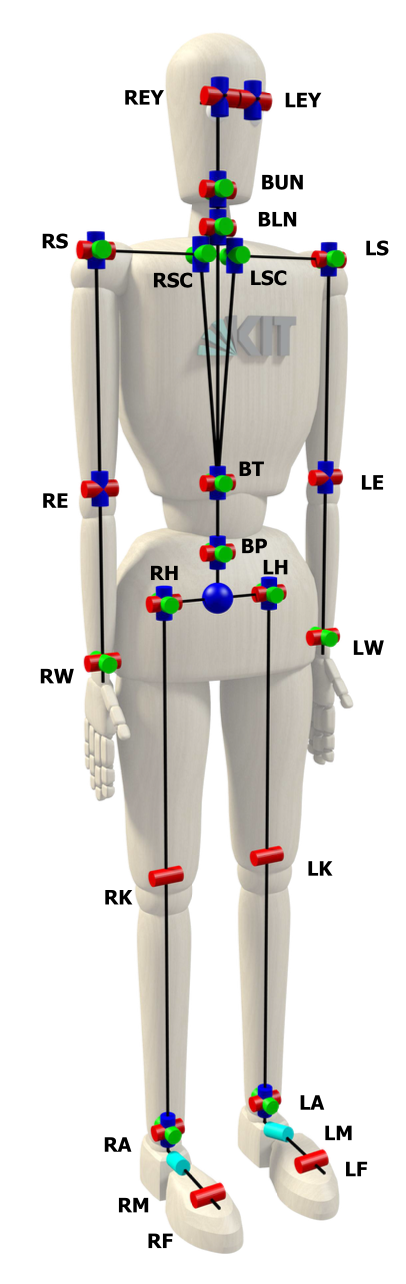
\includegraphics[width=.32\textwidth]{img/mmm-model.png}
				\caption{The base of the mmm model as in \cite{Plappert2016}}
				\label{fig:mmm-model}
			\end{center}
		\end{wrapfigure}
		As mentioned in the introductory part of this chapter, the KIT Motion-Language dataset\cite{Plappert2016} will be used, and in this section, the relevant information about it will be discussed. This dataset was first assembled to link human motions to the natural language, which is of huge interest for the generation of semantic presentations of human activities. In addition to that, this dataset would be instrumental in implementing learning machines capable of generating robot activities based on natural language input\cite{Plappert2016}. The team responsible for the KIT Motion-Language Database has developed the tools to aggregate the data from multiple motion capture databases and included the results in their database using a unified representation outlined in \ref{subsec:mmm-notation}. According to the team, the dataset contains a total of 3911 motions totaling 11.23 hours of motion capturing duration\cite{Plappert2016}.
		\subsection{mmm-Notation} \label{subsec:mmm-notation}
			The information about the motions in this dataset is persistently stored as xml-files using the mmm-notation ensuring the ease of reusability and the portability of these files. For this notation, the mmm (Master Motor Map) was developed which is a framework and toolkit for capturing, representing, and reproducing human motion. In this thesis, only the representing part is relevant for extracting the information about the position of the joints the velocity and the root joint position for example\cite{mmm2014}. The xml-based mmm-notation is made of two parts. First, the setup of the model with the necessary information to recreate the motion itself, such as the height and the mass of the human, which is stored in the xml-element \textit{ModelProcessorConfig}. In addition to that the joints are defined in the xml-element \textit{JointOrder} and its child elements. Relevant here are the motion frames stored as \textit{MotionFrames}, where the information about the frames of the motions are stored as the children of the \textit{MotionFrames} xml-element:
			\begin{itemize}
				\item The time step of the frame in \textit{Timestep} xml-element.
				\item The root joint positions in each frame in the \textit{RootPosition} xml-element.
				\item The root rotations in each frame in the \textit{RootRotation} xml-element.
				\item Information about the joints sorted according to the joint order specified in the \textit{JointOrder} xml-element, and these joints are illustrated in fig \ref{fig:mmm-model}
				\begin{itemize}
					\item The position of each joint in \textit{rad} in the \textit{JointPosition} xml-element.
					\item Analog to the \textit{JointPosition} xml-element the velocity of each joint is stored in the \textit{JointVelocity} xml-element.
					\item And lastly for the joint acceleration of each joint in the \\\textit{JointAcceleration} xml-element.
				\end{itemize}
			\end{itemize}
			To extract the information stored in these xml-files, the \textit{python} library \\\textit{xml.etree.ElementTree} is used to parse the files. With it the xml-file is parsed and converted into a tree, that can be navigated through iterating over the xml-children of each xml-element until the necessary information is found and extracted either as an attribute of an element or the body of it. These can be ascertained using the \textit{get} or the \textit{text} methods. 
		\subsection{Motion labeling}
			As mentioned in the introductory part of this section, the KIT provided annotations to each motion in this dataset. These annotations are the base for the labeling of each motion, as a class describing and representing the motion as a whole and not describing it in detail. These annotations are a list of sentences describing the motion in multiple turns of phrases. This is useful for generating semantic presentations of human activities, but is irrelevant here. Thus, the natural language processing library \textit{nltk} was used to process these annotations and extract the verbs, and sort them by the frequency of their occurrences.\newline
			The position tagging was achieved by using the average perceptron, which theoretical foundation was outlined in \ref{sec:nlp}. Then, the most frequent verbs are determined and used as labels for the motions where they are part of the assigned annotation. Some verbs, such as be, will, etc..., are for this task marked as stop verbs and discarded. The resulting list of most frequent verbs is \{'walk', 'turn', 'run', 'stand', 'jump', 'wave', 'stumbl', 'danc', 'throw', 'kneel', 'kick'\}. However, the use of stemmer, as explained in \ref{subsec:stemmer}, is paramount to correctly estimate the frequency and to uniformly classify motion, without taking into account the tense and the position of the verb in the annotation.\newline
			\begin{algorithm}[H]
				\caption{The motion labeling algorithm}\label{alg:motionlabeling}
				\KwData{Annotations and motions as a dictionary annotation\_motion}
				\KwResult{Labeled motions as a dictionary motion\_label}
				annotation\_text $\gets$ concat(annotations)\;
				position\_word $\gets$ tag(annotation\_text)\; \Comment{Using the perceptron to determine the position of each word}
				verb\_frequency $\gets$ empty\_dictionary()\;
				\ForEach{word and position in position\_word}{
					\If{position is verb}{
						stem $\gets$ get\_stem(word)\; \Comment{Using the stemmer find the stem of the word}
						\lIf{word in verb\_frequency}{ increment verb\_frequency[stem]}
						\lElse{intialize verb\_frequency[stem] with 1}
					}
				}
				most\_frequent\_verbs $\gets$ get\_most\_frequent(verb\_frequency, 10)\;
				\ForEach{annotation and motion in annotation\_motion}{
					label $\gets$ empty\_list(), labeled $\gets$ False\;
					\ForEach{word in annotation}{
						stem $\gets$ get\_stem(word)\;
						\If{word in most\_frequent\_verbs}{add stem to label\; labeled $\gets$ True\;}
					} \lIf{labeled}{assign label to motion in motion\_label}
				}
			\end{algorithm}
			\begin{figure}[H]
				\centering
				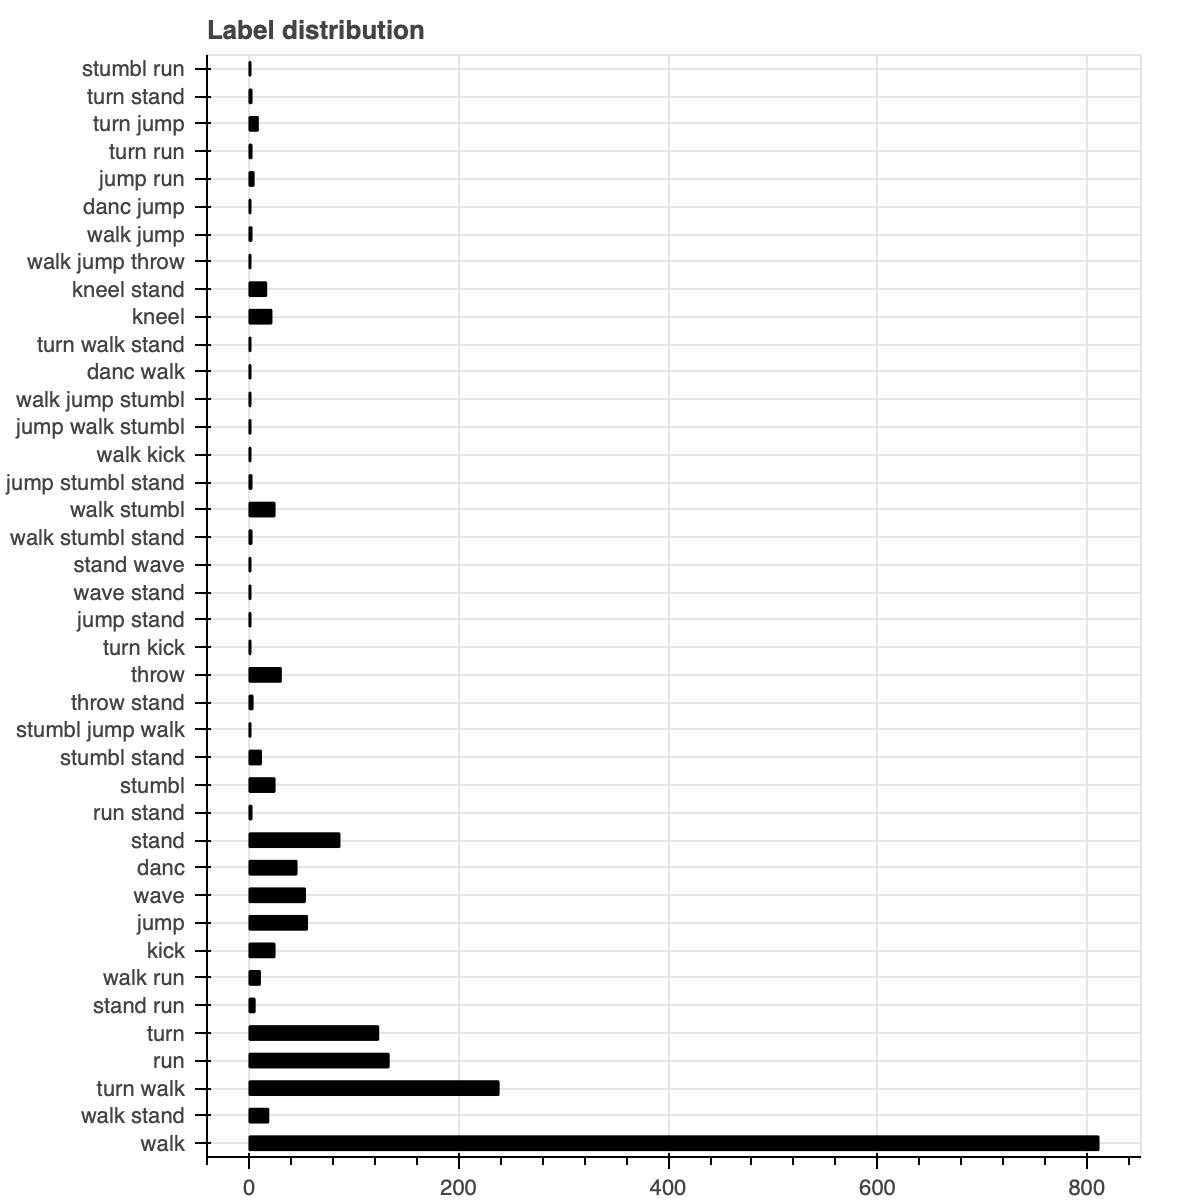
\includegraphics[width=\textwidth]{img/label-distribution.png}
				\caption{Label distribution showing the presence of composite activities in the dataset}
				\label{fig:label-distribution}
			\end{figure}
			In this thesis, the Porter stemmer was used to determine the stem of each verb encountered in all annotations. Lastly, each motion was labeled by the stem of a verb by iterating over the tokens in the annotation and searching for a verb in the most frequent list of verbs calculated beforehand. The motion labeling can be summarized with alg. \ref{alg:motionlabeling}, which was used to label the motions and resulted in the distribution as fig. in \ref{fig:label-distribution}. This process was the result of an improved process, where only the first label was taken. This didn't take into account the composite motion, such as walk then turn and stumble walk then jump, etc.., and made it difficult to train the models and get decent results.\newline
		\subsection{Preliminary Analysis}\label{subsec:preliminary_analysis}
			To assess the usefulness of the dataset the library \textit{Bokeh} some statistical analysis of the dataset must be done. First, the number of motions without annotations must be determined and the affected motions must be discarded. By implementing a downloader object, that extracts the content of the zip file containing the files. Then, the annotations will be checked and determined, if these are empty. A total of 3012 motions were correctly annotated, and the rest was deleted.\newline
			The motions vary in length and the number of frames in them, and in \ref{section:training} some sequential models were used to train the models implemented in \ref{section:learningmachines}, thus the length of the frames must be defined to both ensure taking all the relevant information for the classification and avoid padding the motions too much with zeros. As the number of frames to be fed to the model to generate a prediction of to train it must have a beforehand defined length. The distribution of the number of frames for all motion is visualized in fig \ref{fig:num_frames_distro}. Taking the results of the visualization into account, it has been determined that the length of most motions is around 2000 frames. Thus, this value has been chosen to be the standard input length in \ref{section:learningmachines}.\newline
			\begin{figure}[H]
				\centering
				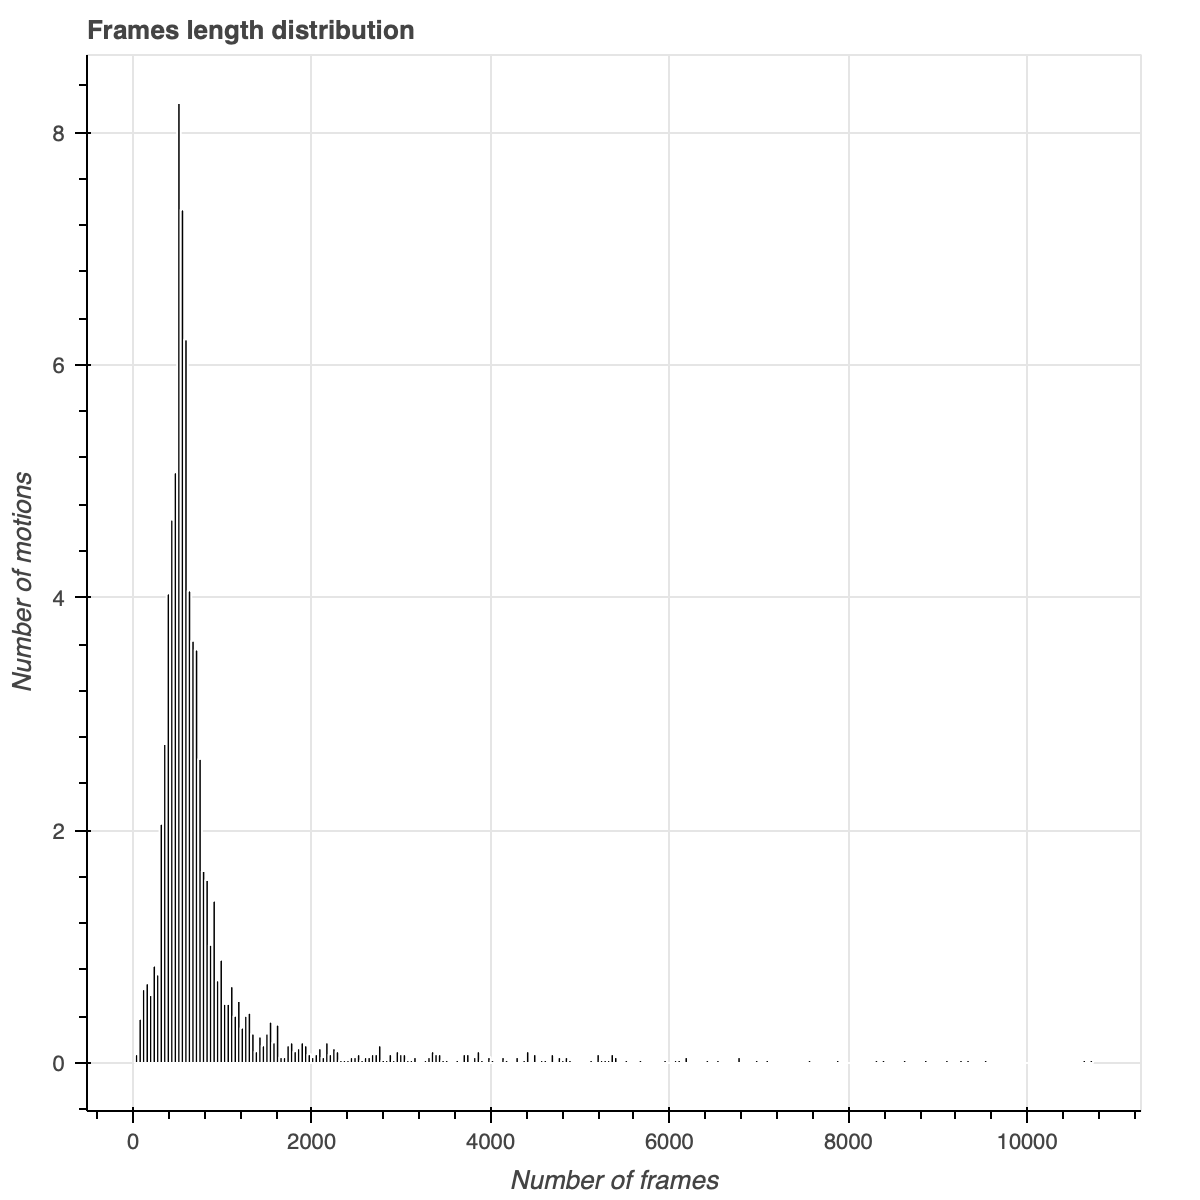
\includegraphics[width=.9\textwidth]{img/num-frames-distro.png}
				\caption{The distribution of the number of frames of motions}
				\label{fig:num_frames_distro}
			\end{figure}
			In addition to that, it has been shown that all the \textit{JointVelocity} and \textit{JointAcceleration} xml-element are all not defined. This makes them irrelevant to this project. In section \ref{section:learningmachines}, only the information stored in \textit{JointPosition}, \textit{RootPosition} and \textit{RootRotation} will be extracted and used in the next steps.
	\section{Pipeline}\label{sec:pipeline}
		 To facilitate and accelerate rapid prototyping it was paramount to divide the process into sizable chunks and persistently store the results of each step on disk. This however would prove to be a difficult endeavor, as it requires more encapsulation of the code and using \textit{numpy} for storing the information extracted from the xml-files. To achieve this, the npy-file format was used to make further processing more robust and optimize the read time and storage.
		\begin{figure}[H]
			\centering
			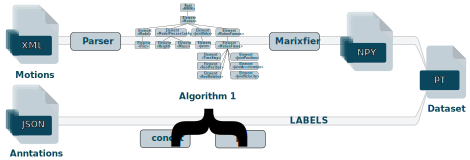
\includegraphics[width=\textwidth]{img/pipeline.pdf}
			\caption{The process of creating the dataset with the information extracted from the KIT Motion-Language dataset}
			\label{fig:pipeline}
		\end{figure}
		As shown in fig \ref{fig:pipeline}, a pipeline was implemented to streamline and accelerate the prototyping process by persistently storing the result of each step on disk. This eliminates the need for repeated parsing and extraction of the information from the xml-files, which is time-consuming and slows down experimenting quite significantly. Firstly, all xml-files are parsed with \textit{ElementTree.xml} and the content of all the \textit{Motion} xml-elements is extracted sequentially and stored in a matrix. Using the \textit{numpy} library these matrices were stored in npy-files to be read in the next pipeline stage. Next, the algorithm \ref{alg:motionlabeling} was implemented to figure out the most frequent verbs and to label each motion by a verb from the set of most frequent verbs. Lastly, the assembled dataset is converted into a \textit{pyTorch} tensor object and stored persistently, in case the next model is able of using the parameters used in the assembly, such as the number of frames, the labels used and the number of features.
	\section{Implementation}
		In this section, the general aspects of the implementation of this project will be outlined. Fig \ref{fig:overview} shows the package UML-diagram for the entire project, which is divided into three main sections.\newline
		\begin{figure}[H]
			\centering
			\includegraphics[width=\textwidth]{img/general_overview.pdf}
			\caption{The general overview of the implementation of the pipeline in fig \ref{fig:pipeline} and the experimentation framework}
			\label{fig:overview}
		\end{figure}
		First, as mentioned in \ref{sec:pipeline} the pipeline is meant to be the groundwork for the facilitation of experimentation and prototyping. For this purpose, the module dataset was written to encapsulate the implementation needed to parse and matrixify the xml-files, which will be further touched on in \ref{subsec:parser_matrixifier}. Next, a base implementation for all learning machines must be implemented, where the training and evaluation process is implemented. As such, the user won't need to replicate the implementation of a new learning machine is added to the suite of models available for experimentation. More about this will be mentioned in the next section \ref{subsec:models}. Lastly, the module experiment will be the base for experimentation and prototyping, where the models and the context of an experiment are specified in json-file. Then, an experiment is initialized and run generating a visualization summarizing basic information about the performance of the trained model and visualizing the training process and validation results. This will be the subject in the last subsection of this section.
		\subsection{Parser and Matrixifier}\label{subsec:parser_matrixifier}
			With the module \textit{dataset.py} the dataset is assembled, and the motions are labeled. First, the class \textit{MotionDataset} is responsible for downloading the dataset from the wen and extracting its content in a target folder, where all future operations will be performed. Next, the xml-files are parsed and the extracted information stored in the xml-elements \textit{MotionFrame} are combined and assembled in matrices and then stored as npy-files. This can be triggered using the parse method of this class, which comes with some optional keyword arguments to tweak its behavior accordingly. As illustrated in fig \ref{fig:parsermatrixifier}, this class comes with following methods:
			\begin{description}
				\item[\textit{download}] automates the downloading of the KIT dataset from the website of the team and places it in the root directory, where all the generated data from the KIT dataset will be stored.
				\item[\textit{extract}] extract the zip-file downloaded by \textit{download} and places the files in the same directory.
				\item[\textit{parse}] is the workhorse of this class and is the method responsible for parsing the xml-files and extracting the data in the \textit{MotionFrame} xml-element. This method creates a \textit{Motion} object for each motion and adds it to its list of motions. Next, this method calls the parse method of the class \textit{Motion} to trigger the parsing and creation of npy-files. If the flag \textit{train} is set, the labels for each motion are generated based on a pre-defined set of stems as outlined in \ref{alg:motionlabeling}. 
			\end{description}
			\begin{figure}[H]
				\centering
				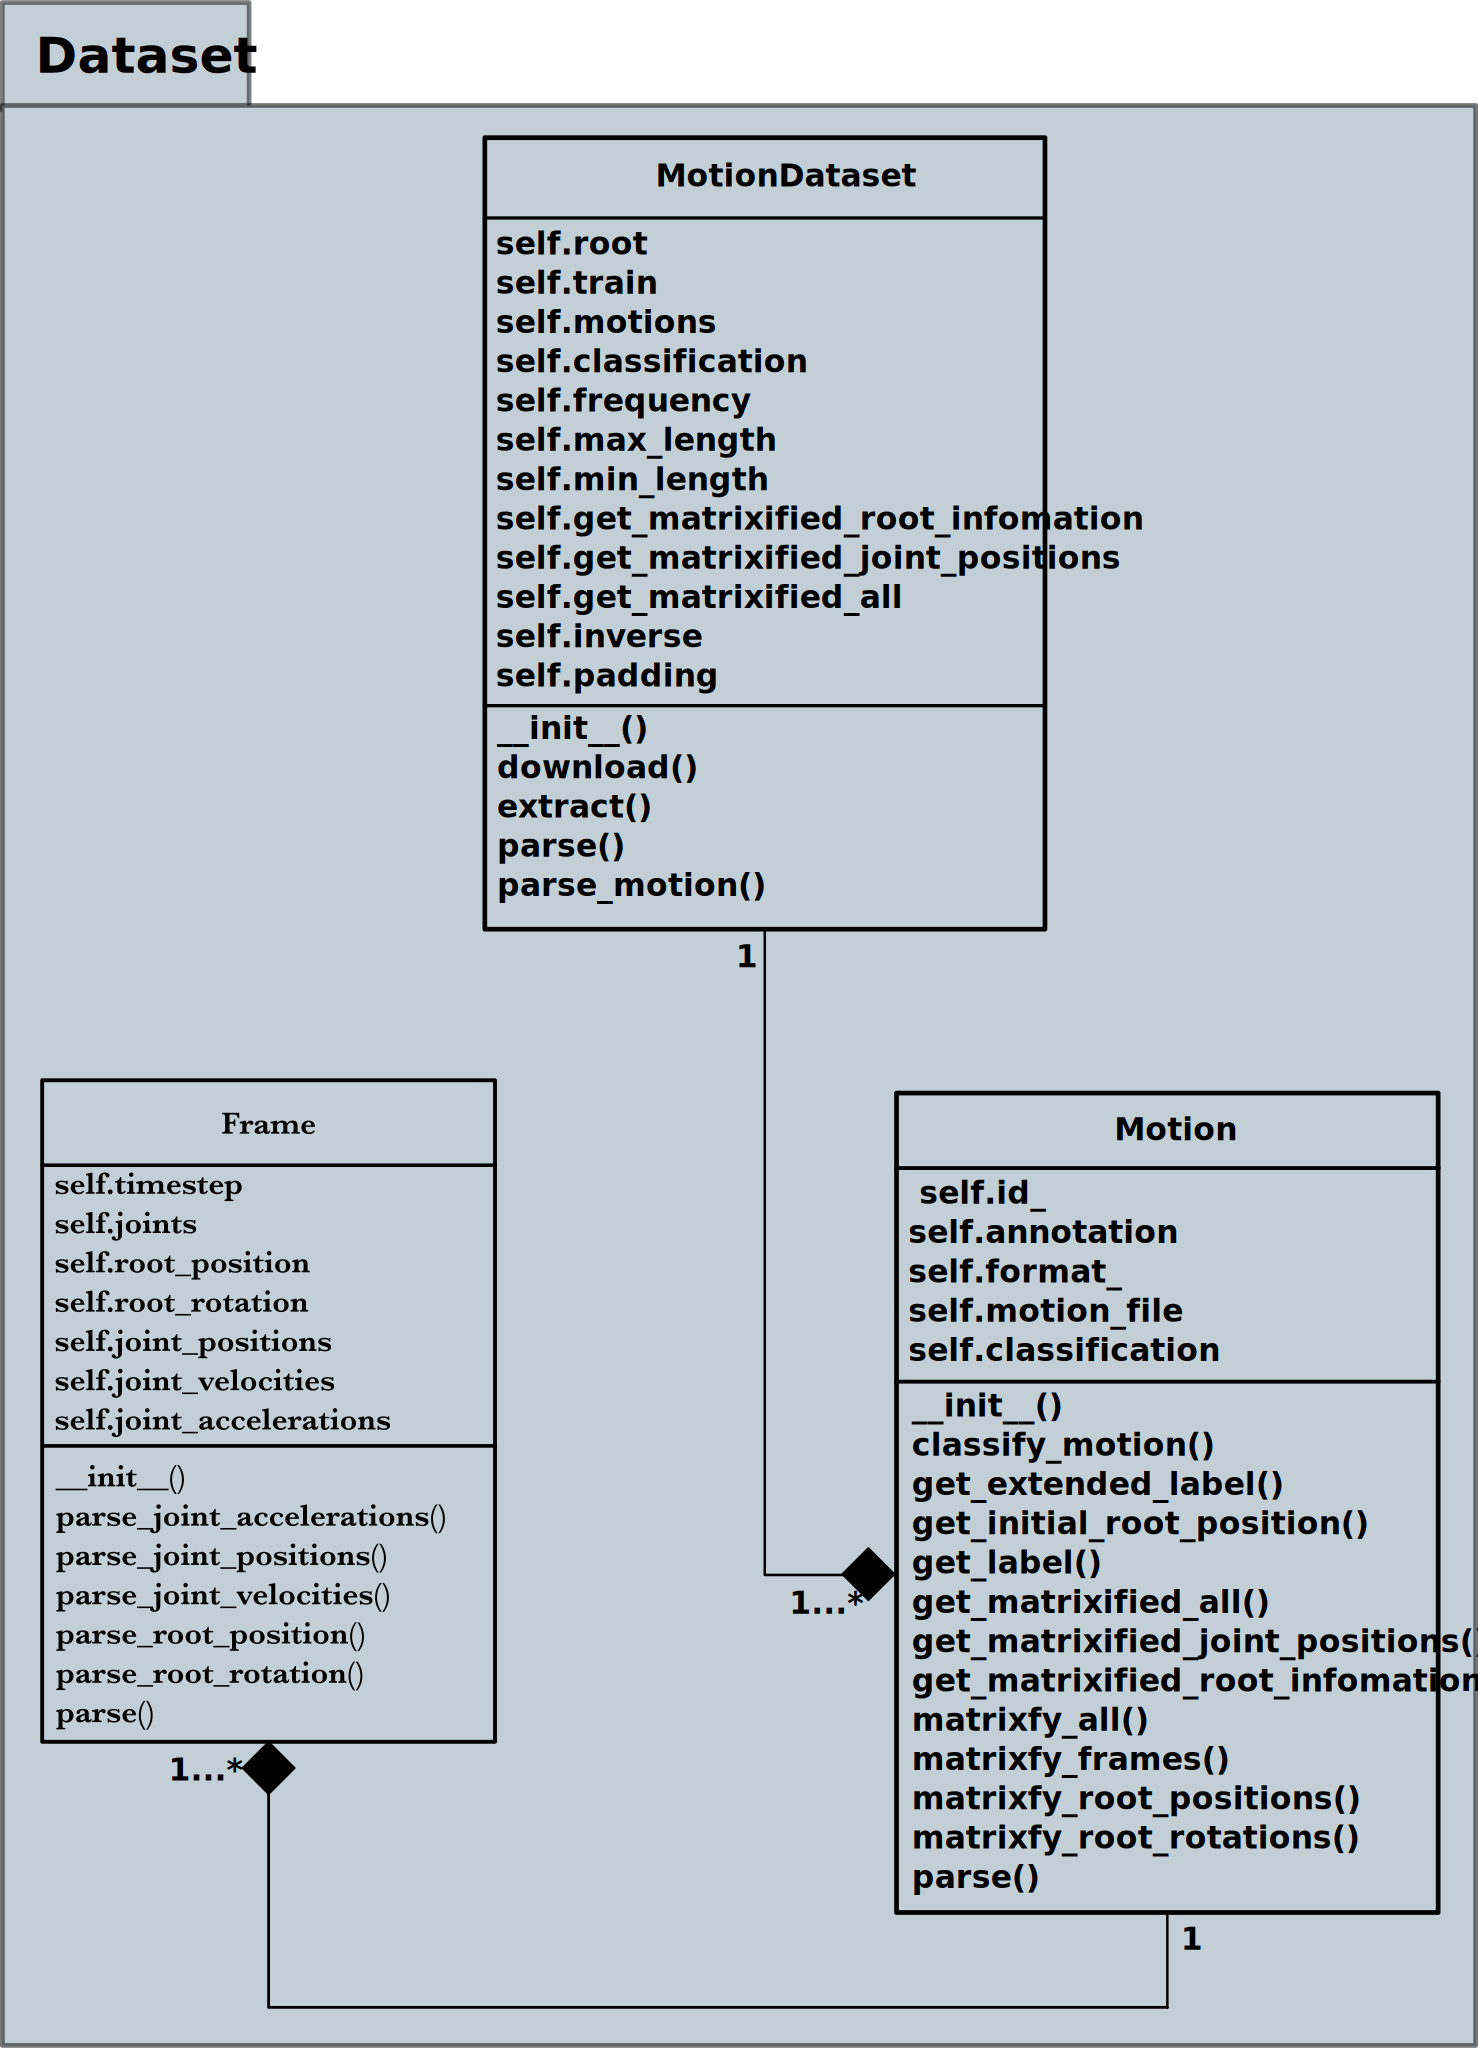
\includegraphics[width=.7\textwidth]{img/parser_matrixfyer_architecture.pdf}
				\caption{The implementation of the parser and matrixfier}
				\label{fig:parsermatrixifier}
			\end{figure}
			As a result of Each \textit{MotionDataset} object encapsulate a set of \textit{Motion} objects. The class \textit{Motion} is the one implementing the parsing of each motion and the labeling process with the following methods:
			\begin{description}
				\item[\textit{classify\_motion}] iterates through the annotations provided to each motion and checks the appearance of the stems predefined in the corresponding \textit{MotionDataset} object. Here, two approaches were implemented, where in the first the motion is labeled with the first appearing stem in the annotation. This might increase the number of motions used in the training process. However, it might introduce conflicting data to the model and lead to more confusion, where these motions represent composite activities. The other approach is to check for the appearance of the stems in the entire annotation and label motions with composite labels if more than one stem appeared in the annotation.
				\item[\textit{parse}] uses the \textit{xml.ElementTree.etree} library to parse to xml-files and extracts information about motion, such as the weight and the height of the participant. The resulting xml-tree is then passed to the \textit{matrixfy\_*} for further processing.
				\item[\textit{matrixfy\_*}] are the methods responsible for creating \textit{Frame} objects encapsulating the information about each frame in the motion. These \textit{Frame} objects extract the data from the xml-Elements and prepare them for matrixfication, where for example the positions of the joints are stored as character sequences and need to be split and typecast to be used in the next step of this process. Lastly, the extracted data is stored in npy-files.
				\item[\textit{get\_matrixfied\_*}] read the npy-files stored by \textit{matrixfy\_*} and apply some transformations to them to make them suitable for the training process. An example of that would be padding to make all motions uniformly long or remove some frames if the length of the motion exceeds the specified maximum length of frames. In addition to that, the implementation allows for using a frequency to shorten the motions by setting a frequency. With a frequency of 5 only every fifth frame is taken, and the rest are discarded.
			\end{description}
			The user of the pipeline can exactly specify the information extracted from the xml-files. This makes it more possible to experiment and even expand the experiments to include more information like the \textit{JointVelocity}, which wasn't specified in the xml-files and was set to 0. First, using the \textit{get\_matrixfied\_*} with the suffix \textit{root\_information} takes only the information stored in the xml-elements related to the root elements, such as \textit{RootPosition} and \textit{RootRotation}. Next, the suffix \textit{joint\_information} specifies that only the information related to the joints is used. However, this is only limited to the joints positions as all other xml-elements beside \textit{JointPosition} like \textit{JointVelcity} are unspecified as mentioned earlier. Lastly, using the \textit{all} suffix specifies that all information must be extracted and combined into a matrix, which is then used in the next step.
		\subsection{Models}\label{subsec:models}
			Now, the data is available and various learning machines can be trained on it. However, learning machines have common tasks and implementations such as the training and valuation processes. These algorithms generally only differ in how the \textit{forward} method is implemented. This is a very promising venue, as an implementer can specify the behavior of the objects representing the learning machines in a base class and then specify the behavior of the \textit{forward} method in child classes for each concrete learning machine. With this intuition, the module \textit{models} can be divided into two main parts. First, the base class \textit{Model} specifies the \textit{fit} and \textit{validate} methods. On the other hand, the child classes specify the constructor to each leaning machine, i.e. how many layers the models have and their inner components, and the \textit{forward} method. These are the methods describing the general behavior implemented in these classes and further information are illustrated in the class diagram in fig \ref{fig:models_implementation}.
			\begin{figure}[H]
				\centering
				\includegraphics[width=.7\textwidth]{img/models_implementation.pdf}
				\caption{Implementation of the models module}
				\label{fig:models_implementation}
			\end{figure}
		\subsection{Experiment}
			The goal of implementing the module \textit{experiment} is as mentioned earlier to speed up the evaluation and prototyping process. Here, the user can specify an experiment by using json-files, to clean up the code and prevent bloats in the code base. The last is a direct consequence of the direct implementation of each experiment, where only one or two parameters are changed, such as the frequency and the maximum and minimum number of frames allowed in all motions. The objects representing these experiments are dictionaries having two sections:
			\begin{description}
				\item[\textit{params}] contains the parameter of the dataset, such as the frequency and which information is then taken to assemble the dataset. In addition to that, the assembling process is also specified with a set of flags. For example, by setting flag \textit{oversample} to true the instances of underrepresented classes in the dataset are duplicated for the purpose of rebalancing the class distribution for the imbalanced dataset. 
					\begin{itemize}
						\item "frequency",
						\item "min\_length",
						\item "max\_length",
						\item "get\_matrixified\_root\_infomation",
						\item "get\_matrixified\_joint\_positions",
						\item "get\_matrixified\_all",
						\item "padding": "zero"|"last",
						\item "inverse": setting it to true reverses the order of frames,
						\item "oversample": use the oversampling algorithms to balance the dataset,
						\item "normalize": normalize the dataset
					\end{itemize}
				\item[\textit{models}] specifies the models used in the experiments and the training parameters. Some of these parameters are optional and only used for recurrent neural networks.
					\begin{itemize}
						\item "model": the class of the model,
						\item "device": the device used for the training, which an depend on the machine used for the training.
						\item "learning\_rate": the learn rate used in the training process.
						\item "num\_epochs": the number of epochs used for the training of the learning machine,
						\item optional "hidden\_size",
						\item optional "num\_layers",
						\item optional "bidirectional"
					\end{itemize}
			\end{description}
			This automated experimenting process was further expanded to allow for automated experimentation in the parameters of the dataset, as these are set for each experiment. To make this possible, the \textit{ExperimentSet} interface was implemented to facilitate the conception and running of multiple experiments. In the json-data adding a new experiment set with particular parameters of the dataset involves only appending these to the list available there. In addition to that, in each experiment, a set of stems used as labels is specified in a separate json-file to ensure that they can be used by multiple experiment sets and reduce redundancy.\newline
			\begin{figure}[H]
				\centering
				\includegraphics[width=.35\textwidth]{img/experiment_implementation.pdf}
				\caption{The implementation of the experiment module}
				\label{fig:experiement_implementation}
			\end{figure}
			Next, an \textit{ExperimentSet} is initialized and parametrized with the information in the json-file then run by the method \textit{run}, where each experiment is executed and the model pertaining to it initialized. Lastly, a visualization of the results of the validation of the models in the experiment and stored in an html-file using the \textit{bokeh} visualization library. The details of the implementation is illustrated in fig. \ref{fig:experiement_implementation} as a uml package diagram.
	\section{Learning Machines}
		\label{section:learningmachines}
		For the propose of training and evaluating the results of each learning machine used in this thesis. The MLP (Multilayer Perceptron) and the CNN (Convolutional Neural Network) have been used as a baseline to be compared. At first, it was assumed that a dedicated model for sequential input, such as RNN (Recurrent Neural Networks), GRU (Gated Recurrent Units) and LSTM (Long Short Term Memory), would prove more performant than the baseline, but this was in most cases not true. In this section, the implementation of the used learning machines will be discussed in further detail. To achieve this the machine learning library \textit{pytorch} was used, as it is a well-documented and accessible library suitable for the goals and aspirations of this thesis. To experiment with models, the implementation should be flexible, as in the number of features could vary according to the number of features extracted. The implementation of the extraction of the information about the frames of a motion is done in the following three cases:
		\begin{enumerate}
			\item Extracting only the information about the root joint, i.e. the rotation and the position in space.
			\item Extracting only the information about the joints, i.e. the rotation of each joint on an axis.
			\item Extracting all the information available in the xml-files.
		\end{enumerate}
		The result is a sequence of vectors containing the information, that is then used to train the model or to generate a prediction.\newline
		First, a very simple MLP (Multilayer Perceptron) was implemented. To experiment with it, it has been trained using the three cases as outlined before. This will demonstrate if the models would perform better with more features. The architecture of the model is illustrated in fig. \ref{fig:wang2017timemlp}. As a baseline, a CNN (Convolutional Neural Network) was also used. These models proved to be good varying degrees, and the results of their training will be discussed in \ref{chap:evaluation}. Next, RNNs as more suitable models for time series classification tasks, but with different flavors to gauge the performance of other variants of recurrent networks, that try to overcome the inherent problems with them outlined in \ref{subsec:rnns}.
	\section{Training}\label{section:training}
		Now, the models can be trained, but some inherent problems of HAR (Human Activity Recognition) come to light as outlined in \ref{subsec:probHAR}. An example of that would be the fact that the generated, as illustrated in \ref{fig:label-distribution}, is highly unbalanced. A solution would be using a weighted loss function, where a miss classification of a less represented activity would lead to a higher loss value. This can be directly implemented, where using the native loss function \textit{cross\_entropy}. This loss function already incorporated the use of the weights. Nevertheless, the user must calculate these weights by using the frequency rate of each class and figure them out accordingly. For class \textit{c} with a frequency rate \textit{n} and \textit{N} the number of instances in the datasets, the weight for the class \textit{c} would be $w=n/N$. Another approach would be the oversampling for less represented classes and/or the undersampling of highly represented classes, this is a naive approach and has some serious consequences on the performance of the trained models. On one hand, removing samples from the dataset is a counter to the fact that the more data a model has for training the better these models generalize. And on the other hand, oversampling will quite probably lead to the overfitting of the models after the training process and will add more computational overhead to it. Concretely, the number of instances of a less dominant class is used to calculate the duplication rate of each class to make the number of instances of each class equal.\newline
		However, the dataset generated in this project is very peculiar and doesn't take into account a lot of the problems outlined there. This is a direct consequence of the methods used here to label the data and compile the dataset, which were particularly error-prone and made the results achieved extremely questionable. The results of training the models implemented in this project and more will be documented in the next chapter \ref{chap:evaluation}.
